\documentclass{article}[a4paper]
\usepackage[a4paper, left=2.5cm,right=2cm,top=2.5cm,bottom=2.5cm]{geometry}
\usepackage[utf8]{inputenc}
\usepackage{csquotes}
\usepackage{booktabs}
\usepackage{amsmath}
\usepackage{mathtools}% http://ctan.org/pkg/mathtools
\usepackage{caption}
\captionsetup{width=.75\textwidth}
\usepackage[usestackEOL]{stackengine}
\usepackage{float}
\usepackage{subcaption}
\usepackage{tikz}
\usetikzlibrary{shapes.geometric,arrows,positioning,fit}
\usetikzlibrary{shapes,calc,arrows}
\usepackage{natbib}
\usepackage{graphicx}
\usepackage{subfiles}
\usepackage{blindtext}
\usepackage{hyperref}
\usepackage{float}
\usepackage{physics} % for 'pdv' macro
\usepackage{qtree}
\usepackage{stmaryrd}
\usepackage{multicol}
\usepackage{xparse}
\usepackage{amssymb}
\usepackage{xcolor}
\usepackage{neuralnetwork}
\usepackage{pgfplots}
\usepackage{sidecap}
 \usepackage{listings}
\usepackage{tikz}
\usepackage{xcolor}

\usetikzlibrary{decorations.pathreplacing}

\pgfplotsset{compat=1.16}

% Syntax: \colorboxed[<color model>]{<color specification>}{<math formula>}
\newcommand*{\colorboxed}{}
\def\colorboxed#1#{%
  \colorboxedAux{#1}%
}
\newcommand*{\colorboxedAux}[3]{%
  % #1: optional argument for color model
  % #2: color specification
  % #3: formula
  \begingroup
    \colorlet{cb@saved}{.}%
    \color#1{#2}%
    \boxed{%
      \color{cb@saved}%
      #3%
    }%
  \endgroup
}

\def\XXX#1{\textcolor{red}{XXX #1}}

\NewDocumentCommand{\codeword}{v}{%
\texttt{\textcolor{blue}{#1}}%
}
\newcommand\Mycomb[2][^n]{\prescript{#1\mkern-0.5mu}{}C_{#2}}
\def\XXX#1{\textcolor{red}{XXX #1}}
\newcommand{\vect}[1]{\boldsymbol{\textcolor{blue}{#1}}}

\title{\textbf{Elements of Machine Learning}\\
Assigment 1 - Problem 6
}
\author{ Sangeet Sagar(7009050), Philipp Schuhmacher(7010127)\\
        \texttt{\{sasa00001,phsc00003\}@stud.uni-saarland.de}
}
% \pgfplotsset{compat=1.17}
% \parindent 0in
% \parskip 0em
\begin{document}
\maketitle
\section*{Part 1}
It's inaccurate to say that relationship between all variables are linear. A variety of relationship can be visualized in the scatter plot among different variables.
\begin{enumerate}
    \item No relationship: Some variables hold no relationship. E.g.\texttt{mpg-origin}, \texttt{cylinders-origin},\\ \texttt{displacement-origin}. Or rather increase or decrease of one variable is independent of other.
    \item Linear Relationship: Some variables are linearly correlated like \texttt{displacement, horsepower, and weight}. These variables are \textbf{strongly correlated}.
    \item Non-linear relationship: A few variables are non-linearly connected like \texttt{mpg} is non-linearly related with \texttt{weight}, \texttt{horsepower} and \texttt{displacement}. We can also call these \textbf{negatively correlated}.
    \item Scattered points: These are just scattered points and the connection between the variables could not be determined. E.g. \texttt{acceleration}-\texttt{mpg}. These variables are \textbf{weakly correlated}. \texttt{acceleration}-\texttt{weight}.
\end{enumerate}

\begin{figure}[H]
    \centering
    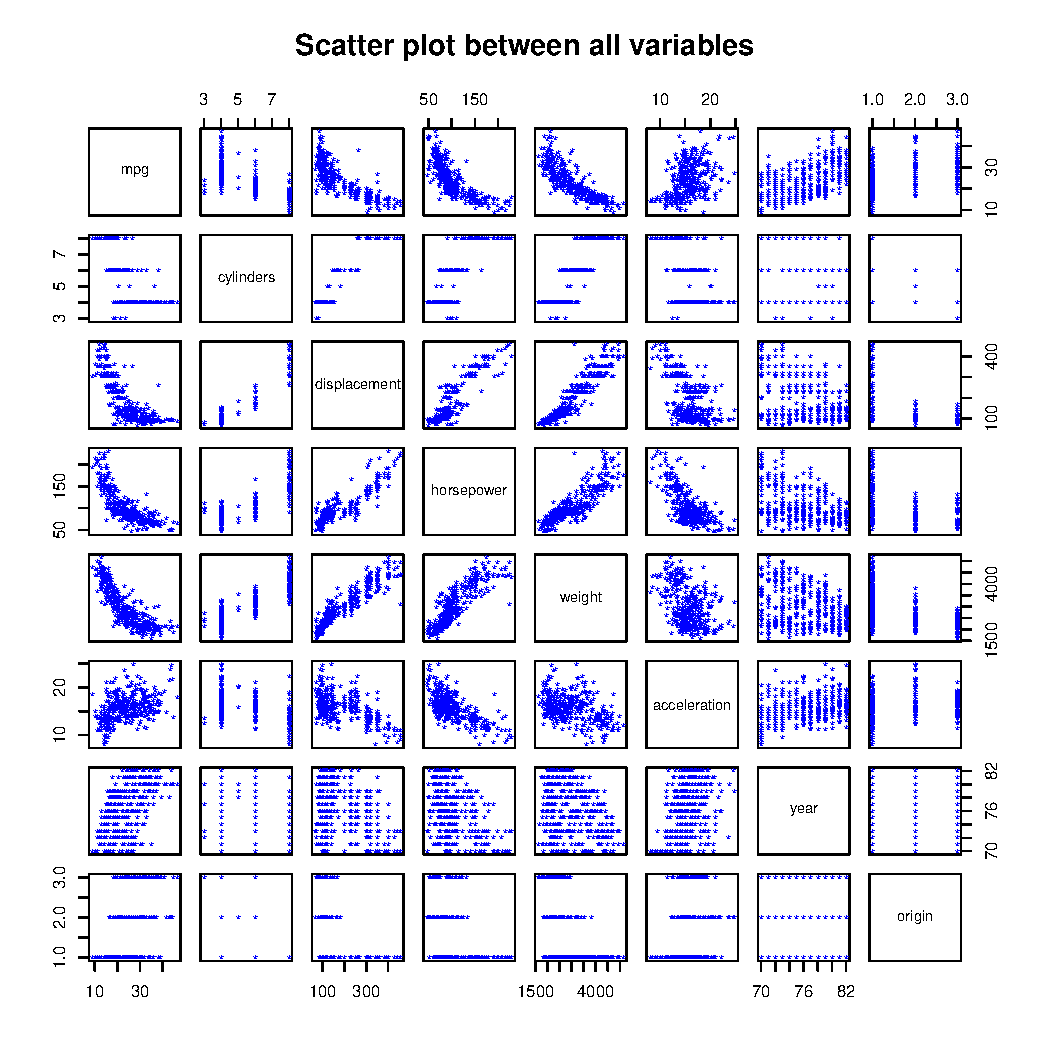
\includegraphics[width=6in]{HW1/rplot.pdf}
    \caption{Scatterplot between all variables namely \texttt{mpg, cylinders, displacement, horsepower, weight, acceleration, year, origin}}
\end{figure}

\section*{Part 2}
Two variables that appear to be the most highly
\begin{enumerate}
    \item \textbf{Correlated}: \texttt{cylinder-displacement}, \texttt{weight-displacement}. However a few other pairs like \texttt{horsepower}-\texttt{displacement} and \texttt{weight-cylinder} also appear to be equally highly co-related. Its difficult to differentiate visually. By looking at graph, the data points in all of these pairs strictly follow a positive linear behaviour. 
    \item \textbf{Anti-correlated}: \texttt{mpg-displacement} and \texttt{mpg-weight} appear to be most highly anti-correlated variables because of their inverse relationship. \texttt{mpg-cylinder}, \texttt{mpg-horsepower} also appear to be anti-correlated on a similar extent, but the negative non-linearity was more obvious in the former.
\end{enumerate}
Using the \texttt{cor()}, we find that 
\begin{enumerate}
    \item \texttt{cylinder-displacement}, \texttt{weight-displacement} are the most highly correlated variables with scores of 0.950 and 0.93 respectively.
    \item \texttt{mpg-displacement} and \texttt{mpg-weight} are the most anit-correlated variables with with scores of -0.80 and -0.832 respectively.
\end{enumerate}
Thus, the results from \texttt{cor()} are almost same as what can be visualized with slight variations. However, a close inspection of the scatter plot makes it clear. The goal here is to observe for variable pairs that show strong positive linear behaviour (highly correlated) and those that show strong linear/non-linear behaviour (highly anti-correlated).

\section*{Part 3}
In order to determine a statistically significant predictors, we need to look for variables with high absolute t-value as well as small p-value. The small p-value indicates a stronger evidence that we should reject the null hypothesis and that there is an relation that holds between predictor and response.
\begin{lstlisting}
                     Estimate     Std. Error      t value     Pr(>|t|)
    cylinders        -3.558078    0.1456755       -24.42468   1.311384e-80
    displacement     -0.06005143  0.002240043     -26.80815   1.660642e-90
    horsepower       -0.1578447   0.006445501     -24.48914   7.031989e-81
    year             1.230035     0.08735748      14.08048    1.075794e-36
\end{lstlisting}
\textcolor{red}{Which predictors appear to have a statistically significant relationship to the outcomes?}\\
Each predictor appears to hold statistically significant relationship with the response for the reason that $p$-value for each predictor is less that $5\%$.
% As can be concluded from the above table that \texttt{cylinder} is not significant in determining the target response \texttt{mpg} because it has highest p-value of 0.0499. While other predictors like \texttt{displacement, horsepower, year} are significant in the above multiple regression model.
\begin{lstlisting}
                    R2 score 
    cylinders       0.604689
    displacement    0.6482294
    horsepower      0.6059483
    year            0.3370278
\end{lstlisting}
\textcolor{red}{How good are the resulting models?}\\
All of the resulting model fit the data except one. The extent of fit is similar among predictors like \texttt{cylinders, displacement, horsepower} fitting almost $60\%$ of the data. However \texttt{year} gives a fit with only $33\%$ of the data, hence the resulting model with this predictor is not good.


\section*{Part 4}
\textcolor{red}{How is the model fit? (using $R^2$)?}\\
The $R^2$ statistic is a measure of the linear relationship between the response and the predictor. Using multiple linear regression, the $R^2$ value is observed to be $0.809$, which suggests that the $80\%$ of the data fits the regression model. This score is, in fact, higher than each model in part 3. Therefore, the multiple linear regression fits the given data well than a linear regression using a single predictor.

\begin{lstlisting}
Coefficients:
                  Estimate   Std. Error      t value     Pr(>|t|)
(Intercept)  -1.453525e+01 4.7638818940  -3.05113578 2.437741e-03
cylinders    -3.298591e-01 0.3321041332  -0.99323994 3.212169e-01
displacement  7.678430e-03 0.0073577361   1.04358597 2.973318e-01
horsepower   -3.913556e-04 0.0138365215  -0.02828425 9.774501e-01
weight       -6.794618e-03 0.0006700227 -10.14087727 1.416190e-21
acceleration  8.527325e-02 0.1020355670   0.83572081 4.038303e-01
year          7.533672e-01 0.0526181480  14.31763010 1.410428e-37

R-sq value:[1] 0.8092553
\end{lstlisting}

\textcolor{red}{What can you observe in the different models concerning the significance of the relationship between response and individual predictors?}\\
Predictors like \texttt{cylinders, displacement, horsepower, acceleration} have $p$-value more than $5\%$; hence they are non-significant, and there does not exist any substantial relationship between the response and these individual predictors. However, other predictors like \texttt{weight, year} have $p$-value less than $5\%$, thus, supporting the evidence that the null hypothesis be rejected since there is some significant association between the response and these individual predictors.
\\~\\
\textcolor{red}{What does the sign of the coefficient (i.e. of the estimate) tell you about the relationship between the predictor and the response?}\\
The sign of the coefficient, i.e. $t$-value, tells us about the direction of the effect the predictor is having on the response \texttt{mpg}. If the sign is positive, it means that the response will increase with the increase in that individual predictor (keeping other predictors as constant) and vice-versa.


\section*{Part 5}
\textcolor{red}{Identify the residual plot.}\\
First plot i.e Residual vs Fitted is the residual plot
\\~\\
\textcolor{red}{Does the residual plot suggest any non-linearity in the data (provide an explanation)? Does the residual plot suggest an unusually large outliers?}\\
Looking the residual plot, it can be concluded that there is no specific pattern, While a curve in the pattern can been but the residuals are scattered. Hence, it indicates of the non-linearity in the data.\\
Outliers can be inferred form the  Residual vs Leverage plot. The red dashed line at the top-right suggests that there exists an unusually large outlier but could not be detected in the plot. Hence their inclusion or exclusion will affect the model.


\begin{figure}[H]
    \centering
    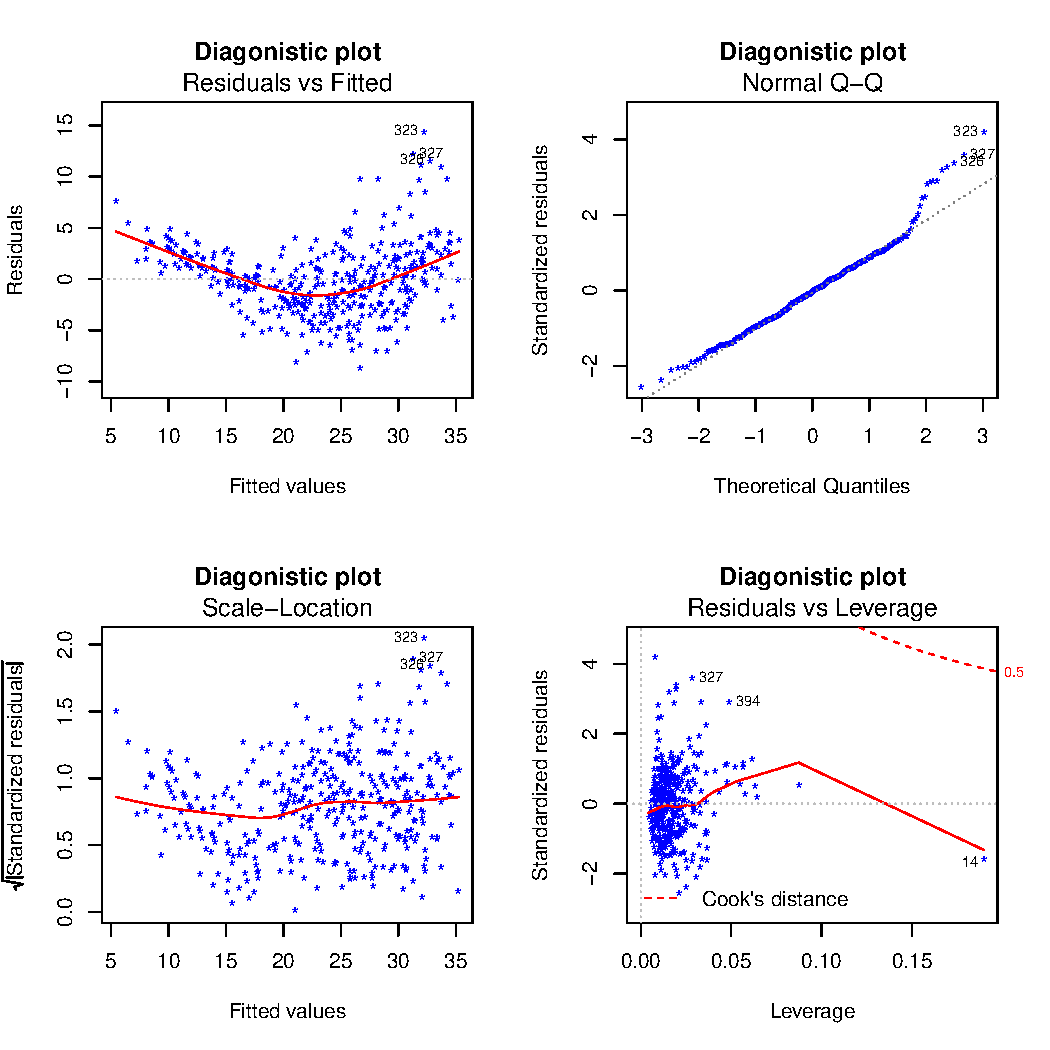
\includegraphics[width=6in]{HW1/diagplot.pdf}
    \caption{Diagonistic plots}
\end{figure}

\bibliographystyle{plainnat}
\bibliography{references}
\end{document}